\documentclass[12pt]{report}
\usepackage{scribe,graphicx,graphics}
\usepackage{float}
\usepackage{siunitx}
\usepackage{braket}
\usepackage{mathabx}
\usepackage{listings}
\usepackage[bbgreekl]{mathbbol}
\course{CSE 389D} 	
\coursetitle{Mathematical Modeling}	
\semester{Spring 2025}
\lecturer{} % Due Date: {\bf Mon, Oct 3 2016}}
\lecturetitle{Problem Set}
\lecturenumber{5}   
\lecturedate{}    
\usepackage{enumerate}
\newcommand{\remind}[1]{\textcolor{red}{\textbf{#1}}} %To remind me of unfinished work to fix later
\newcommand{\hide}[1]{} %To hide large blocks of code without using % symbols

\newcommand{\ep}{\varepsilon}
\newcommand{\vp}{\varphi}
\newcommand{\lam}{\lambda}
\newcommand{\Lam}{\Lambda}
%\newcommand{\abs}[1]{\ensuremath{\left\lvert#1\right\rvert}} % This clashes with the physics package
%\newcommand{\norm}[1]{\ensuremath{\left\lVert#1\right\rVert}} % This clashes with the physics package
\newcommand{\floor}[1]{\ensuremath{\left\lfloor#1\right\rfloor}}
\newcommand{\ceil}[1]{\ensuremath{\left\lceil#1\right\rceil}}
\newcommand{\A}{\mathbb{A}}
\newcommand{\B}{\mathbb{B}}
\newcommand{\C}{\mathbb{C}}
\newcommand{\D}{\mathbb{D}}
\newcommand{\E}{\mathbb{E}}
\newcommand{\F}{\mathbb{F}}
\newcommand{\K}{\mathbb{K}}
\newcommand{\N}{\mathbb{N}}
\newcommand{\Q}{\mathbb{Q}}
\newcommand{\R}{\mathbb{R}}
\newcommand{\T}{\mathbb{T}}
\newcommand{\X}{\mathbb{X}}
\newcommand{\Y}{\mathbb{Y}}
\newcommand{\Z}{\mathbb{Z}}
\newcommand{\As}{\mathcal{A}}
\newcommand{\Bs}{\mathcal{B}}
\newcommand{\Cs}{\mathcal{C}}
\newcommand{\Ds}{\mathcal{D}}
\newcommand{\Es}{\mathcal{E}}
\newcommand{\Fs}{\mathcal{F}}
\newcommand{\Gs}{\mathcal{G}}
\newcommand{\Hs}{\mathcal{H}}
\newcommand{\Is}{\mathcal{I}}
\newcommand{\Js}{\mathcal{J}}
\newcommand{\Ks}{\mathcal{K}}
\newcommand{\Ls}{\mathcal{L}}
\newcommand{\Ms}{\mathcal{M}}
\newcommand{\Ns}{\mathcal{N}}
\newcommand{\Os}{\mathcal{O}}
\newcommand{\Ps}{\mathcal{P}}
\newcommand{\Qs}{\mathcal{Q}}
\newcommand{\Rs}{\mathcal{R}}
\newcommand{\Ss}{\mathcal{S}}
\newcommand{\Ts}{\mathcal{T}}
\newcommand{\Us}{\mathcal{U}}
\newcommand{\Vs}{\mathcal{V}}
\newcommand{\Ws}{\mathcal{W}}
\newcommand{\Xs}{\mathcal{X}}
\newcommand{\Ys}{\mathcal{Y}}
\newcommand{\Zs}{\mathcal{Z}}
\newcommand{\ab}{\textbf{a}}
\newcommand{\bb}{\textbf{b}}
\newcommand{\cb}{\textbf{c}}
\newcommand{\db}{\textbf{d}}
\newcommand{\ub}{\textbf{u}}
\newcommand{\sbb}{\textbf{s}}
%\renewcommand{\vb}{\textbf{v}} % This clashes with the physics package (the physics package already defines the \vb command)
\newcommand{\wb}{\textbf{w}}
\newcommand{\xb}{\textbf{x}}
\newcommand{\yb}{\textbf{y}}
\newcommand{\zb}{\textbf{z}}
\newcommand{\vbb}{\textbf{v}}
\newcommand{\Ab}{\textbf{A}}
\newcommand{\Bb}{\textbf{B}}
\newcommand{\Cb}{\textbf{C}}
\newcommand{\Db}{\textbf{D}}
\newcommand{\eb}{\textbf{e}}
\newcommand{\ex}{\textbf{e}_x}
\newcommand{\ey}{\textbf{e}_y}
\newcommand{\ez}{\textbf{e}_z}
\newcommand{\zerob}{\mathbf{0}}
\newcommand{\abar}{\overline{a}}
\newcommand{\bbar}{\overline{b}}
\newcommand{\cbar}{\overline{c}}
\newcommand{\dbar}{\overline{d}}
\newcommand{\ubar}{\overline{u}}
\newcommand{\vbar}{\overline{v}}
\newcommand{\wbar}{\overline{w}}
\newcommand{\xbar}{\overline{x}}
\newcommand{\ybar}{\overline{y}}
\newcommand{\zbar}{\overline{z}}
\newcommand{\Abar}{\overline{A}}
\newcommand{\Bbar}{\overline{B}}
\newcommand{\Cbar}{\overline{C}}
\newcommand{\Dbar}{\overline{D}}
\newcommand{\Ubar}{\overline{U}}
\newcommand{\Vbar}{\overline{V}}
\newcommand{\Wbar}{\overline{W}}
\newcommand{\Xbar}{\overline{X}}
\newcommand{\Ybar}{\overline{Y}}
\newcommand{\Zbar}{\overline{Z}}
\newcommand{\Aint}{A^\circ}
\newcommand{\Bint}{B^\circ}
\newcommand{\limk}{\lim_{k\to\infty}}
\newcommand{\limm}{\lim_{m\to\infty}}
\newcommand{\limn}{\lim_{n\to\infty}}
\newcommand{\limx}[1][a]{\lim_{x\to#1}}
\newcommand{\liminfm}{\liminf_{m\to\infty}}
\newcommand{\limsupm}{\limsup_{m\to\infty}}
\newcommand{\liminfn}{\liminf_{n\to\infty}}
\newcommand{\limsupn}{\limsup_{n\to\infty}}
\newcommand{\sumkn}{\sum_{k=1}^n}
\newcommand{\sumk}[1][1]{\sum_{k=#1}^\infty}
\newcommand{\summ}[1][1]{\sum_{m=#1}^\infty}
\newcommand{\sumn}[1][1]{\sum_{n=#1}^\infty}
\newcommand{\emp}{\varnothing}
\newcommand{\exc}{\backslash}
\newcommand{\sub}{\subseteq}
\newcommand{\sups}{\supseteq}
\newcommand{\capp}{\bigcap}
\newcommand{\cupp}{\bigcup}
\newcommand{\kupp}{\bigsqcup}
\newcommand{\cappkn}{\bigcap_{k=1}^n}
\newcommand{\cuppkn}{\bigcup_{k=1}^n}
\newcommand{\kuppkn}{\bigsqcup_{k=1}^n}
\newcommand{\cappk}[1][1]{\bigcap_{k=#1}^\infty}
\newcommand{\cuppk}[1][1]{\bigcup_{k=#1}^\infty}
\newcommand{\cappm}[1][1]{\bigcap_{m=#1}^\infty}
\newcommand{\cuppm}[1][1]{\bigcup_{m=#1}^\infty}
\newcommand{\cappn}[1][1]{\bigcap_{n=#1}^\infty}
\newcommand{\cuppn}[1][1]{\bigcup_{n=#1}^\infty}
\newcommand{\kuppk}[1][1]{\bigsqcup_{k=#1}^\infty}
\newcommand{\kuppm}[1][1]{\bigsqcup_{m=#1}^\infty}
\newcommand{\kuppn}[1][1]{\bigsqcup_{n=#1}^\infty}
\newcommand{\cappa}{\bigcap_{\alpha\in I}}
\newcommand{\cuppa}{\bigcup_{\alpha\in I}}
\newcommand{\kuppa}{\bigsqcup_{\alpha\in I}}
\newcommand{\Rx}{\overline{\mathbb{R}}}
\newcommand{\dx}{\,dx}
\newcommand{\dy}{\,dy}
\newcommand{\dt}{\,dt}
\newcommand{\dax}{\,d\alpha(x)}
\newcommand{\dbx}{\,d\beta(x)}
\DeclareMathOperator{\glb}{\text{glb}}
\DeclareMathOperator{\lub}{\text{lub}}
\newcommand{\xh}{\widehat{x}}
\newcommand{\yh}{\widehat{y}}
\newcommand{\zh}{\widehat{z}}
\newcommand{\<}{\langle}
\renewcommand{\>}{\rangle}
\renewcommand{\iff}{\Leftrightarrow}
\DeclareMathOperator{\im}{\text{im}}
\let\spn\relax\let\Re\relax\let\Im\relax
\DeclareMathOperator{\spn}{\text{span}}
\DeclareMathOperator{\sym}{\text{Sym}}
\DeclareMathOperator{\myskew}{\text{Skew}}
\DeclareMathOperator{\Re}{\text{Re}}
\DeclareMathOperator{\Im}{\text{Im}}
\DeclareMathOperator{\diag}{\text{diag}}
\endinput
\usepackage{xcolor}
\definecolor{codegreen}{rgb}{0,0.6,0}
\definecolor{codegray}{rgb}{0.5,0.5,0.5}
\definecolor{codepurple}{rgb}{0.58,0,0.82}
\definecolor{backcolour}{rgb}{0.95,0.95,0.92}

\lstdefinestyle{mystyle}{
    backgroundcolor=\color{backcolour},   
    commentstyle=\color{codegreen},
    keywordstyle=\color{magenta},
    numberstyle=\tiny\color{codegray},
    stringstyle=\color{codepurple},
    basicstyle=\ttfamily\footnotesize,
    breakatwhitespace=false,         
    breaklines=true,                 
    captionpos=b,                    
    keepspaces=true,                 
    numbers=left,                    
    numbersep=5pt,                  
    showspaces=false,                
    showstringspaces=false,
    showtabs=false,                  
    tabsize=2
}

\lstset{style=mystyle}
\usepackage{amsthm}
\newtheoremstyle{custom}
  {\topsep} % Space above
  {\topsep} % Space below
  {\upshape} % Body font
  {} % Indent amount
  {\itshape} % Theorem head font
  {.} % Punctuation after theorem head
  { } % Space after theorem head
  {} % Theorem head spec
\theoremstyle{custom}
\newtheorem{case}{Case}

% Insert your name here!
\scribe{Student Name: Noah Reef}
\newcommand{\rb}{\bold{r}}

\begin{document}
\maketitle

\section*{Problem 5.1}
\subsection*{Part a}

\begin{equation*}
 E = -\frac{\hbar^2}{2(M/2)} \frac{\partial^2}{\partial d^2} + \frac{e^2}{4\pi \epsilon_0 d} + \epsilon(d) 
\end{equation*}

\subsection*{Part b}
Let 
\begin{align*}
  \epsilon_a &= 2\left(\epsilon_{1s} - \frac{\gamma - \beta}{1 - S}\right) \\
  \epsilon_b &= 2\left(\epsilon_{1s} - \frac{\gamma + \beta}{1 + S} \right)\\
\end{align*}
where
\begin{align*}
  S &= \left(1 + \frac{d}{a_0} + \frac{d^2}{3a_0^2}\right)e^{-d/a_0} \\
  \gamma &= E_{HA} \left[\frac{a_0}{d} - \left(1 + \frac{a_0}{d}\right)e^{-2d/a_0}\right] \\
  \beta &= E_{HA} \left(1 + \frac{d}{a_0}\right)e^{-d/a_0}
\end{align*}
\subsection*{Part c}
Recall that the effective potential energy is given by
\begin{equation*}
V_p(d) = \frac{e^2}{4\pi \epsilon_0 d} + \epsilon(d) = \frac{a_0E_{HA}}{d} + \epsilon(d) = \frac{a_0E_{HA}}{d} + 2\left(\epsilon_{1s} - \frac{\gamma \pm \beta}{1 \pm S}\right)
\end{equation*}
note that we can rewrite this as
\begin{equation*}
\frac{V_p(d)}{E_{HA}} = \frac{a_0}{d} - 1 - 2\frac{\gamma \pm \beta}{E_{HA}(1 \pm S)} = -1 + \frac{a_0}{d} - \frac{\frac{a_0}{d} - \left(1 + \frac{a_0}{d}\right)e^{-2d/a_0}\pm \left(1 + \frac{d}{a_0}\right)e^{-d/a_0}}{1 \pm \left(1 + \frac{d}{a_0} + \frac{d^2}{3a_0^2}\right)e^{-d/a_0}}
\end{equation*}

\subsection*{Part d}
\begin{figure}[H]
  \centering
  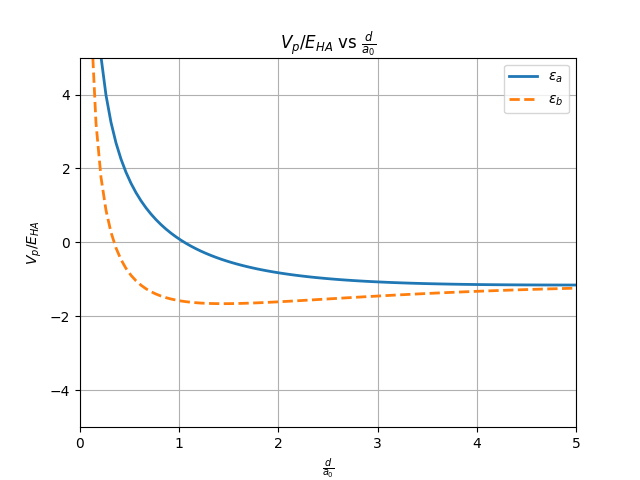
\includegraphics[scale=0.8]{/Users/nreef/Desktop/Spring_2025/hw5_q1_d.png}
\end{figure}

\subsection*{Part e}
We find that the minimum of the effective potential for the bonding case occurs at $d/a_0 = 1.446$ and thus at $d = 1.446a_0$. Then recalling that $a_0 \approx 0.5291 \AA$, we get $d \approx 0.765$ which is about $+1.9 \%$ of the experimental value of $d = 0.75 \AA$.

\subsection*{Part f}
We have that
\begin{equation*}
  \frac{V_p(\infty)}{E_{HA}} = -1 \quad \text{and} \quad \frac{V_p(\text{min})}{E_{HA}} = -1.657
\end{equation*}
and thus the dissociation energy is given by
\begin{equation*}
  \frac{D}{E_{HA}} = \left|\frac{V_p(\infty)}{E_{HA}} - \frac{V_p(\text{min})}{E_{HA}}\right| = |-1 - (-1.657)| = 0.657 \implies D = 0.657E_{HA} \approx 17.88\si{eV}
\end{equation*}
which we get that is about $+295 \%$ of the experimental value of $D = 4.52 \si{eV}$.

\section*{Problem 5.2}
\subsection*{Part a}
Consider the apporximation for the factorial of a large number $n$:
\begin{equation*}
n! \approx (2\pi n)^{1/2}\left(\frac{n}{e}\right)^n \left(1 + \frac{1}{12n}\right)
\end{equation*}
then we see that
\begin{align*}
  \log(n!) &\approx \frac{1}{2}\left[\log(2\pi) + \log(n)\right] + n\left[\log(n) - \log(e)\right] + \log\left(1 + \frac{1}{12n}\right)
\end{align*}
then we get that 
\begin{equation*}
  \frac{\partial}{\partial n} \log(n!) \approx \frac{1}{2n} + [\log(n) - \log(e)] + 1 + \frac{-\frac{1}{12n^2}}{1 + \frac{1}{12n}} = \log(n) - \frac{1 - 12n}{24n^2 + 2n}
\end{equation*}

\subsection*{Part b}
\begin{figure}[H]
  \centering
  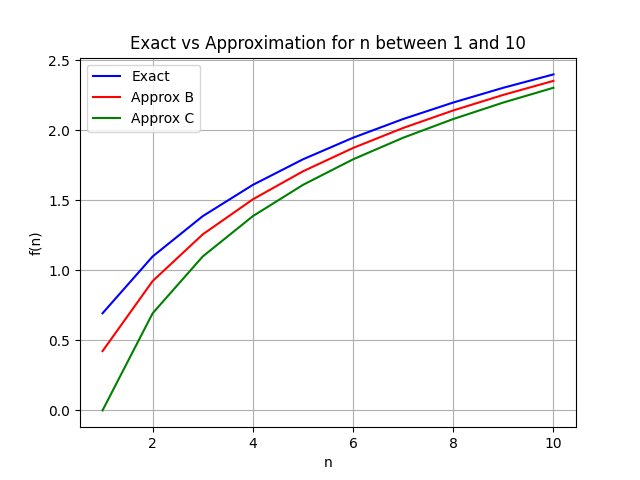
\includegraphics[scale=0.8]{~/Desktop/Spring_2025/CSE_389D/ps_5/hw5_q2_n_10.png}
\end{figure}

% \lstinputlisting[language=python]{~/Desktop/Spring_2025/CSE_389D/ps_5/hw5_q2_b.py}

\subsection*{Part c}
\begin{figure}[H]
  \centering
  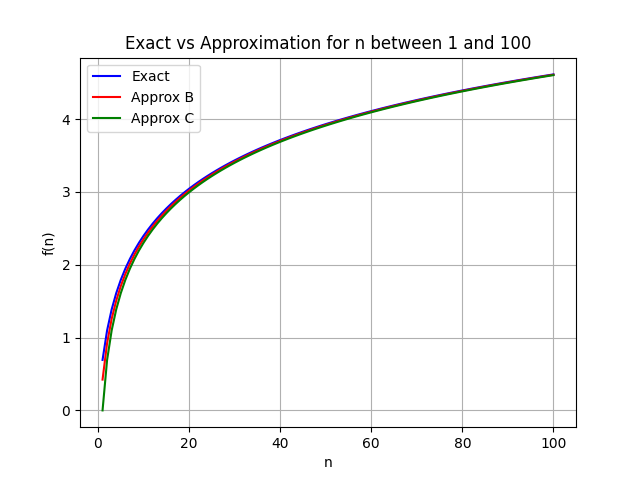
\includegraphics[scale=0.8]{~/Desktop/Spring_2025/CSE_389D/ps_5/hw5_q2_n_100.png}
\end{figure}

% \lstinputlisting[language=python]{~/Desktop/Spring_2025/CSE_389D/ps_5/hw5_q2_c.py}

\section*{Problem 5.3}
\subsection*{Part a}
Recall that the ideal gass law is given by
\begin{equation*}
  PV = N k_B T
\end{equation*}
where $k_B = 1.38064852 \times 10^{-23} \si{J/K}$ is the Boltzmann constant. With the radius of a proton being roughly $r_p \approx 0.85 \times 10^{-15} \si{m}$ we get that the volume of the proton to be $V_p = \frac{4}{3} \pi r_p^3 \approx 2.57244 \times 10^{-45} \si{m^3}$. 
Lastly if we assume that we are at room temparute $T = 293\si{K}$, then we can compute the pressure as
\begin{equation*}
 P = \frac{N k_B T}{V} = 3\frac{1.38064852 \times 10^{-23} \si{J/K} \cdot 293 \si{K}}{2.57244 \times 10^{-45} \si{m^3}} = 4.717 \times 10^{24} \si{Pa}
\end{equation*}

\subsection*{Part b}
From the paper they find that the peak pressure is on the order of $10^{35} \si{Pa}$ which is about $11$ order of magnitudes larger than result seen in part a.

\subsection*{Part c}
A couple assumptions made by the ideal gass law that can be responsible for the difference in findings, is that the ideal gass law assumes that there is no collisions between particles as well as collisions between the containers surface is perfectly elastic. 

\subsection*{Part d}
\begin{equation*}
\Tilde{f}(v) = \left(\frac{2}{\pi}\right)^{1/2} \left(\frac{m}{k_BT}\right)^{3/2} v^2 \exp\left(-\frac{mv^2}{2k_BT}\right)
\end{equation*}
then we see that 
\begin{align*}
  \langle v^2 \rangle &= \int_0^\infty v^2 \Tilde{f}(v) \, dv =\left(\frac{2}{\pi}\right)^{1/2} \left(\frac{m}{k_BT}\right)^{3/2} \int_0^\infty v^4 \exp\left(-\frac{mv^2}{2k_BT}\right) \, dv 
\end{align*}
letting $u^2 = \frac{mv^2}{2k_BT}$ we get that 
\begin{align*}
  \langle v^2 \rangle &=\left(\frac{2}{\pi}\right)^{1/2} \left(\frac{m}{k_BT}\right)^{3/2} \left(\frac{2k_BT}{m}\right)^2 \left(\frac{2k_BT}{m}\right)^{1/2}\int_0^\infty u^4 \exp\left(-u^2\right) \, du \\
  &=4\sqrt{2}\left(\frac{2}{\pi}\right)^{1/2} \left(\frac{k_BT}{m}\right) \frac{3\sqrt{\pi}}{8} = 3\left(\frac{k_BT}{m}\right)
\end{align*}
now since $(\Delta v)^2 = \langle v^2 \rangle - \langle v \rangle^2$ we get that
\begin{equation*}
  (\Delta v)^2 =3\left(\frac{k_BT}{m}\right) - 4\left(\frac{2}{\pi} \frac{k_BT}{m}\right) \implies \Delta v = \sqrt{3-\frac{8}{\pi}}\left(\frac{k_BT}{m}\right)^{1/2}
\end{equation*}
\end{document}
